
\section{Back-of-the-Envelope Cost Benefit Analysis of ABC} \label{appendix:back}

\noindent This section presents a back-of-the-envelope cost-benefit analysis in a similar spirit to that of \citet{Chetty_Friedman_etal_2010_HowDoesYour} and \citet{Kline-Walters_2015_NBER-Evaluating}. The implementation is straightforward and it is based on the argument of  \citet{Chetty_Friedman_etal_2010_HowDoesYour} that a standard deviation in a kindergarten IQ score generates an increase of $13.1\%$ in earnings at age 27.\\

\noindent We perform two exercises. First, one similar to that of \citet{Kline-Walters_2015_NBER-Evaluating}. We calculate the treatment effect of ABC on a kindergarten IQ test---Wechsler Preschool and Primary Scale of Intelligence at Age 5, $\widehat{\Delta}$, and let the (discounted to age 5) life-cycle earnings in 2014 USD dollars be $\$460,793.34$. We take this number straight from \citet{Kline-Walters_2015_NBER-Evaluating}. Based on this, we calculate the total benefits induced by the program as: 

\begin{equation}
B = 460,793.34 \left( \widehat{\Delta} R_{IQ}  N_{\text{Treated}}  -  N_{\text{Control}} \right) , 
\end{equation}

\noindent where $N_{\text{Treated}}$ is the number of subjects in the treatment group and $N_{\text{Control}}$ is the number of subjects in the control group. $R_{IQ}$ is the earnings return to a standard deviation increase in a kindergarten IQ test---13.1\% in the case of \citep{Chetty_Friedman_etal_2010_HowDoesYour}. Then, we let the total cost of the program (discounted to age 5) be $\$5,893,093.20$, as documented in Appendix~\ref{app:programcosts}. We denote this by $C$.\\ 

\noindent For the program to break-even with respect to costs and benefits, a much higher return to the kindergarten IQ test is needed than the one reported in \citep{Chetty_Friedman_etal_2010_HowDoesYour}, $13.1\%$ vs. $40\%$. Figure~\ref{figure:first} plots the relationship between the $B/C$ and various values of $R_{IQ}$.\\ 

\noindent Next, we perform a similar calculation. Instead of letting $R_{IQ}$ vary, we fix it to $13.1\%$ and let the net present value of earnings over the life cycle vary. For the program to break even, this value needs to be beyond a million dollars (Figure~\ref{figuresecond}). \citet{Kline-Walters_2015_NBER-Evaluating} argue that this value is $\$359,064.50$ for disadvantaged populations in the U.S.

\begin{center}
\begin{figure}[H] 
\caption{Benefit-to-cost Ratio and the Earnings Returns to a Kindergarten IQ Test} \label{figure:first}
\centering
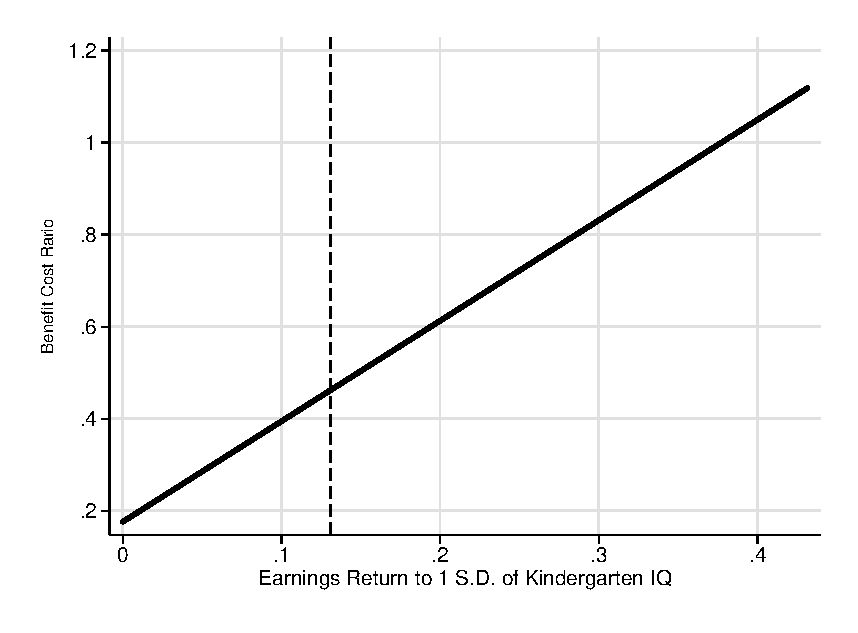
\includegraphics[width=.65\columnwidth]{Output/abc_chettytype_return.eps}
\floatfoot{
\footnotesize
Note: Benefit-to-cost ratio as a function of diverse earnings-returns to a standard deviation of a kindergarten IQ test.
}
\end{figure}
\end{center}

\begin{center}
\begin{figure}[H] 
\caption{Benefit-to-cost Ratio and the Discounted Net Present Value of Earnings}
\label{figuresecond}
\centering
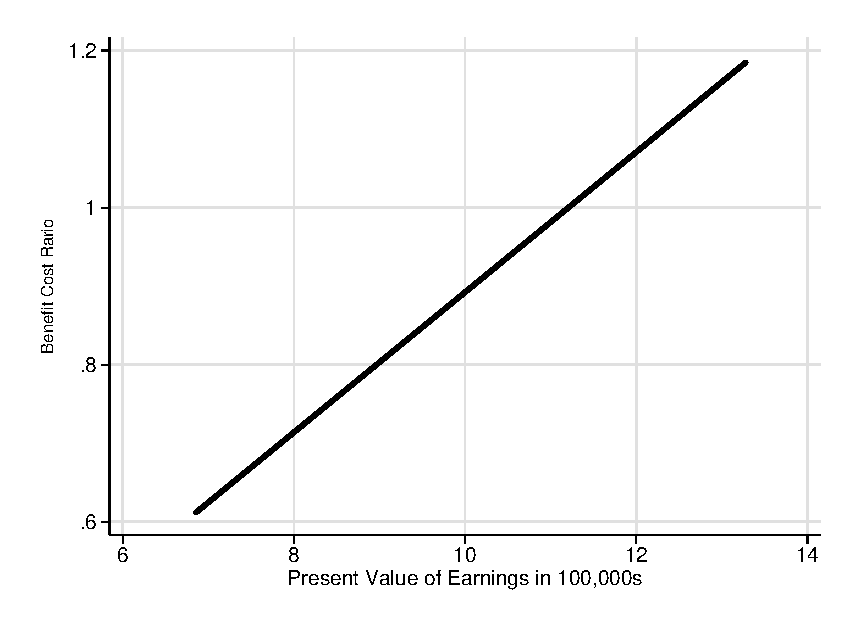
\includegraphics[width=.65\columnwidth]{Output/abc_chettytype_pv.eps}
\floatfoot{
\footnotesize
Note: Benefit-to-cost ratio as a function of diverse net present value of earnings.
}
\end{figure}
\end{center}